\section{Quantifying Power Optimizations}
\label{sec:quantifying}

We consider two related issues in the practical component of our work. The first task is to establish bounds on how much CPU power draw can vary whilst running arbitrary code. This allows us to place an upper limit on how much is possible to optimize a given code by. These bounds also help us tackle a second issue - namely to provide an objective appraisal of the power models proposed elsewhere in the literature.

As previously mentioned, the only property an engineer can influence while optimizing software for reduced power consumption is processor activity factor. As previously discussed, the activity factor of a processor has a linear relationship with dynamic power and secondary non-linear relationships with both static and dynamic power. A developer wishing to save energy should therefore aim to modify their code to reduce its contribution to activity factor.

Although activity factor is defined as a scalar between zero and one, we know that in practice its range will be more limited.  Many logic elements are dedicated to unavoidable tasks which involve frequent state changes, like instruction decoding or clock signalling.This means there will always be some non-zero lower limit to activity factor whilst a processor is active which we label $\alpha$.

Conversely, we know that there is no situation in which any processor will toggle the state of each transistor at every clock signal. Current processors are not physically able to keep all their functional units active simultaneously, which means our upper bound $\beta$ will be significantly lower than unity. More generally we know that any system which toggles every transistor with probability 1 is not capable of performing meaningful computation. We therefore define the range of values that activity factor can feasibly take whilst running a code as $[\alpha  .. \beta]$ where $0 < \alpha < \beta < 1$.

From equations \ref{eq:totpwr}-\ref{eq:leakpwr} we know that, for a fixed platform and temperature, activity factors $\alpha$ and $\beta$ will be associated with constant power draws $P_{\alpha}$ and $P_{\beta}$ respectively, where $P_{\alpha} < P_{\beta}$. The values of these terms are naturally system-dependent and should be determined empirically. 

We are now ready to derive a visual heuristic to guide optimization. We begin by plotting lines with gradients $P_{\alpha}$ and $P_{\beta}$ in \figurename~\ref{fig:modeldraw} to establish a feasible performance envelope. This represents the set of all $(E_\theta, D_\theta)$ pairs for which $P_{\alpha}~<~P_\theta~<~P_{\beta}$, with no bounds placed on runtime, $D_\theta$. It should be clear that all codes,  and by extension their maximally-optimized equivalents, must be represented somewhere within this envelope. We also plot the point which corresponds to our original as $\theta$.

\begin{figure}[ht]                                                               
\centering                                                                      
\lstset{basicstyle=\ttfamily\footnotesize\bfseries,                             
      frame=tb}                                                                 
\lstinputlisting[]{Listings/nops.c}                             
\caption{Baseline Power Micro-Benchmark}                            
\label{fig:microbench}                                                           
\end{figure}  

We approximate $P_{\alpha}$ by monitoring the power consumed whilst running an architecture-specific version of the code given in \figurename~\ref{fig:microbench}. This code performs the least amount of work possible whilst keeping the processor active. It consists of a single instruction, performs no computation and places no demand on the memory subsystems. It is therefore safe to assume that any non-trivial code running on a realistic platform has a higher activity factor than this minimal micro-benchmark. We defer measurement of $P_{\beta}$ for now as its precise value is not relevant to the current discussion.


To constrain our search further we consider the metric we wish to reduce. We know that for two logically equivalent codes $\theta$ and $\lambda$, the transformation $\theta \to \lambda$ is a valid optimization with respect to a cost metric $M$ if and only if $M(\lambda) < M(\theta)$. If we plot the curve linking all points having $M(\lambda) = M(\theta)$, then by definition any optimized versions of $\theta$ can only exist below this line. The exact equation of the curve depends on the metric chosen. We derive the bound for $ED^2P$ below:

\begin{align}
ED^2P(\theta) &= ED^2P(\lambda) \nonumber \\
\Leftrightarrow P_{\theta} \times {D_{\theta}}^{3} &= P_{\lambda} \times {D_{\lambda}}^{3} \nonumber \\
\implies P_{\lambda} &= \frac{P_{\theta} \times {D_{\theta}}^{3}}{{D_{\lambda}}^3} \nonumber \\
\implies E_{\lambda} &= \frac{P_{\theta} \times {D_{\theta}}^{3}}{{D_{\lambda}}^2}
\end{align}

Our final bound considers what it means to optimize code for reduced power draw. We must avoid being too lenient; a large reduction in runtime associated with a negligible reduction in power draw should still be regarded as a classical optimization. On the other hand, our definition should include optimizations which deliver significant reductions in power draw with minuscule reductions in runtime. 

The definition we have settled on is that an optimization $\theta \to \lambda$ is a power optimization with respect to metric $M$ if the change in power draw it delivers is responsible for the majority of the reduction in $M$. Conversely, if the primary benefit of an optimization comes from improved runtime then it is to be considered a runtime optimization. We plot a curve linking those points which have the same ratio of contributions from both power and runtime factors to $M$ as our original code. All valid power optimizations must lie below this so-called contribution bound. Once again the equation for this bound depends on the metric chosen, so we present the derivation for $ED^{2}P$ by way of example:

\begin{align}
\frac{P_{\theta}}{{D_{\theta}}^3} &= \frac{P_{\theta^\prime}}{{D_{\theta^\prime}}^3}\\ 
\implies P_{\lambda} &= \frac{P_{\theta}}{{D_{\theta}}^3} \times {D_{\lambda}}^3 \nonumber \\
\implies E_{\lambda} &= \frac{P_{\theta}}{{D_{\theta}}^3} \times {D_{\lambda}}^4
\end{align}


% All else being equal, energy to solution will reduce if a code can be made to run faster. That said, there is a clear difference between an optimization which specifically targets energy efficiency and this inevitable side-effect of classical optimization.
At first it may appear somewhat academic to base a model on the definition of power optimization. That said, this is an important consideration in practice. Intuitively it makes sense to use the most appropriate tools while searching for optimizations. If code is sub-optimal and the penalty is felt more in one domain than the other then the tools and techniques developed for that domain are better suited to finding the optimization.


\begin{figure}
 
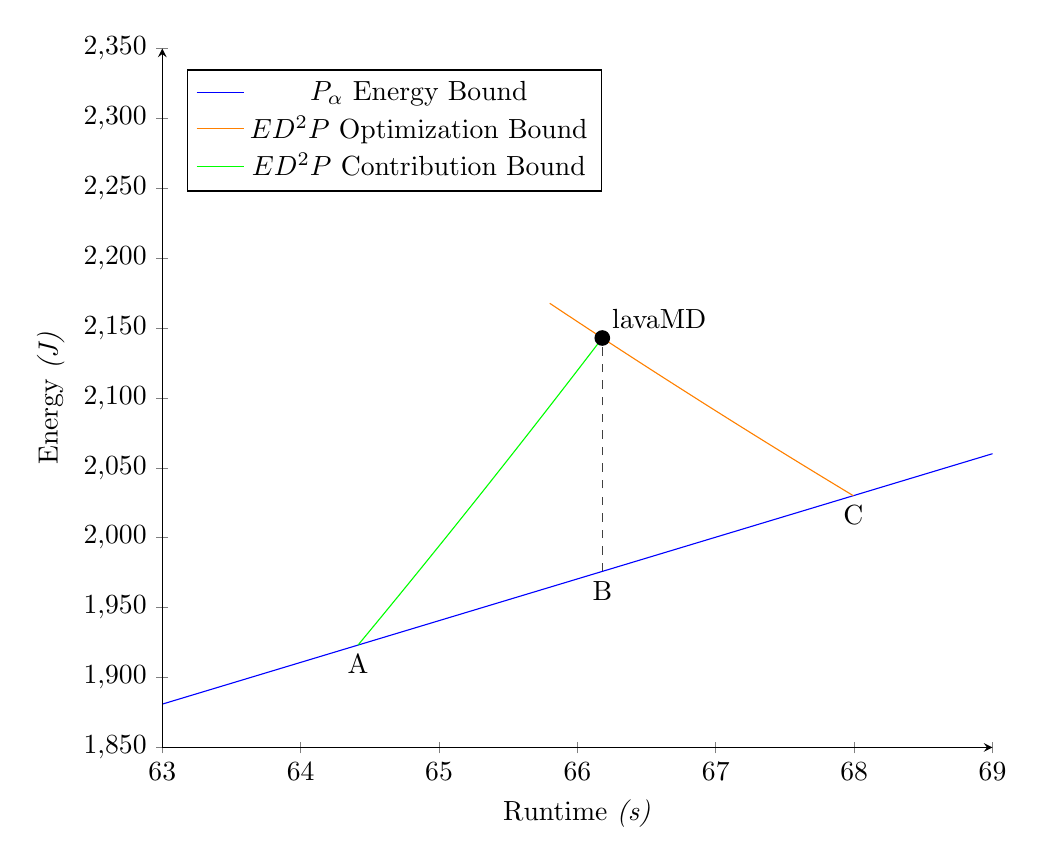
\begin{tikzpicture}
  \begin{axis}[    axis x line=bottom,axis y line=left,
ylabel={Energy \emph{(J)}}, xlabel={Runtime \emph{(s)}}, axis on top,
    xmin=63, xmax=69,
    ymin=1850, ymax=2350,
    width=\linewidth,
    legend style={legend pos=north west}
    ]

    %% Model Parameters %%
    \pgfmathsetmacro{\baselinepower}{29.857} % NOP code, 4 cores, 3.2 ghz
    \pgfmathsetmacro{\codepower}{32.38}
    \pgfmathsetmacro{\codetime}{66.18}
    % Sadly, pgfplots sucks too much to calculate cube roots
    \pgfmathsetmacro{\anodex}{64.4144}
    \pgfmathsetmacro{\anodey}{\anodex * \baselinepower}
    \pgfmathsetmacro{\cnodex}{67.994}
    \pgfmathsetmacro{\cnodey}{\cnodex * \baselinepower}
    \pgfmathsetmacro{\tnodex}{65.8}

    %% Intermezzo Values %%
    \pgfmathsetmacro{\codeenergy}{\codepower * \codetime}
    \pgfmathsetmacro{\baselineenergy}{\baselinepower * \codetime}
    \pgfmathsetmacro{\lowdisplayline}{(2 * \baselinepower + \codepower) / 3}

    % arguments: code power, code time, x - todo, apparently not supposed to do pgfmathparse
    \pgfmathdeclarefunction{metricbound}{3}{%
      \pgfmathparse{((#1 * #2^3) / #3^2)}%
    }
    \pgfmathdeclarefunction{definitionbound}{3}{%
      \pgfmathparse{((#1 / #2^3) * #3^4)}%
    }
     \pgfmathdeclarefunction{optimizationlimits}{3}{%
      \pgfmathparse{(min(metricbound(#1, #2, #3), definitionbound(#1, #2, #3)))}
    }

    % ALPHA BASELINE BOUND 
    \addplot[domain=\pgfkeysvalueof{/pgfplots/xmin}:\pgfkeysvalueof{/pgfplots/xmax},
             blue] {\baselinepower * x};
    \addlegendentry{$P_{\alpha}$ Energy Bound} 
    % BETA ROOFLINE BOUND

    % Constant Time and Power Dashes
    \draw[darkgray, dashed] ({axis cs:\codetime,\baselineenergy}) -- ({axis cs:\codetime,\codeenergy});
 

    \addplot[domain=\tnodex:\cnodex, orange] { metricbound(\codepower, \codetime, x)};
    \addlegendentry{$ED^{2}P$ Optimization Bound}
%
    \addplot[domain=\anodex:\codetime, green] { definitionbound(\codepower, \codetime, x)};
    \addlegendentry{$ED^{2}P$ Contribution Bound}


    \node[circle,fill,inner sep=2pt] at (axis cs:\codetime,\codeenergy) {};
    \node[above right] at (axis cs:\codetime,\codeenergy) {lavaMD};
    
    \node [below] at ({axis cs:\anodex, \anodey}) {A};
    \node [below] at ({axis cs:\codetime,\baselineenergy}) {B};
    \node [below] at ({axis cs:\cnodex, \cnodey}) {C};


 \end{axis}
\end{tikzpicture}

\caption{Code Optimization Space}\label{fig:modeldraw}
\end{figure}


The bounds presented above allow us to identify the area in the Energy/Runtime plane where power-optimized versions of a given code may exist. For the purposes of illustration we add lines of fixed time and power draw based on our initial code measurement. This allows us to subdivide \figurename~\ref{fig:modeldraw} into those areas labelled:

\begin{enumerate}
\centering
\item Power-only optimizations
\item Power-mostly optimizations
\item Time-mostly optimizations
\item Time-only optimizations
\item Code degradation
\end{enumerate}

Only three measurements are required to build this plot; the system's baseline power draw, $P_\alpha$, and the time and energy to solution for the code to be optimized, $D_\theta$ and $E_\theta$ respectively. We can ignore the value of $P_\beta$ when optimizing for power draw as we need not consider any values greater than our initial $P_\theta$.

Despite its simplicity, this technique offers a surprising wealth of information. The vertical distance between $\theta$ and intercept $B$ places an upper limit on the absolute amount of energy which can be saved by power optimization alone. The value $M(\theta) / M(A)$ bounds the amount of improvement in our metric we can expect to see from power optimization. The difference in runtime between intersect $C$ and $\theta$ represents the amount of time we are able to trade off if we hope to achieve a slower yet more energy efficient code. Finally, the value $D(\theta) / D(A)$ represents the smallest speed-up which delivers more benefit than power optimization is capable of.


Having derived our heuristic we set out to apply it to a number of HPC benchmarks. Our first task was to measure the $P_\alpha$ baseline for our test system. This machine incorporates a commodity Intel Ivy Bridge processor which exposes the Running Average Power Limit interface \cite{david:2010aa}. For this reason we chose to use the techniques outlined in \cite{hackenberg:2013aa} to perform our measurements. It is worth noting at this point that our method does not rely on any particular hardware or measurement configurations. The only prerequisites are that the system under test is CMOS-based and accurate power and time measurements are available.

\begin{table}
\centering
\small
\begin{tabular}{@{}ccccc@{}} \toprule
&\multicolumn{4}{c}{CPU Cores Active} \\ \cmidrule(r){2-5}
Frequency (GHz) & 1 & 2 & 3 & 4 \\ \midrule 
1.60 & 9.180 & 10.970 & 12.832 & 14.555 \\ 
1.70 & 9.449 & 11.446 & 13.295 & 15.112 \\ 
1.80 & 9.592 & 11.654 & 13.617 & 15.682 \\ 
1.90 & 9.816 & 12.009 & 14.168 & 16.291 \\ 
2.10 & 10.272 & 12.709 & 15.161 & 17.605 \\ 
2.20 & 10.559 & 13.161 & 15.705 & 18.333 \\ 
2.30 & 10.812 & 13.551 & 16.419 & 19.070 \\ 
2.40 & 11.303 & 14.290 & 17.012 & 19.946 \\ 
2.50 & 11.680 & 14.784 & 18.000 & 20.837 \\ 
2.60 & 11.819 & 15.144 & 18.616 & 21.879 \\ 
2.70 & 12.205 & 15.830 & 19.379 & 22.940 \\ 
2.90 & 13.095 & 17.196 & 21.155 & 25.344 \\ 
3.00 & 13.547 & 18.160 & 22.210 & 26.759 \\ 
3.10 & 14.048 & 18.870 & 23.639 & 28.284 \\ 
3.20 & 14.504 & 19.726 & 24.940 & 29.857 \\ 
\bottomrule
\end{tabular}
   \vspace{0.5\baselineskip}
\caption{Test Platform Base CPU Power (W)}
\label{tab:baseline}
\end{table} 

We measured CPU power draw whilst running our baseline micro-benchmark for each combination of core count and frequency supported by the hardware. The results of this investigation are given in Table \ref{tab:baseline}. We then ran a range of codes from common benchmarking suites, targeting various core counts and system configurations. A small number of results from the Rodinia suite is presented in Table \ref{tab:coderesults}. These results come from runs which were configured to use the maximum frequency and core count possible. Our baseline power draw for this configuration is 29.857 Watts.


\begin{table}
\centering
\small
\begin{tabular}{@{}cccc@{}} \toprule
Code & Runtime (s) & Energy (J) & Power (W) \\ \midrule 
CFD & 29.72 & 933.32 & 31.40  \\ 
Heartwall & 24.62 & 787.17 & 31.97 \\ 
lavaMD & 66.18 & 2142.65 & 32.38 \\ 
leukocyte &  38.92 & 1197.91 & 30.78 \\ 
streamcluster & 33.86 & 1086.77 & 32.10 \\ 
\bottomrule
\end{tabular}
   \vspace{0.5\baselineskip}
\caption{Rodinia Results @ 3.2GHz, 4 Cores}
\label{tab:coderesults}
\end{table} 

Of the codes listed above, lavaMD is the strongest candidate for optimization as it has both the highest power draw at 32.38 Watts and the longest runtime of 66.18 seconds. Naturally, we applied our heuristic to determine just how much scope for power optimization this code offers, as displayed by \figurename~\todo{plotme}


\todo{working point}


\begin{figure}
\label{fig:modelpoints}
 
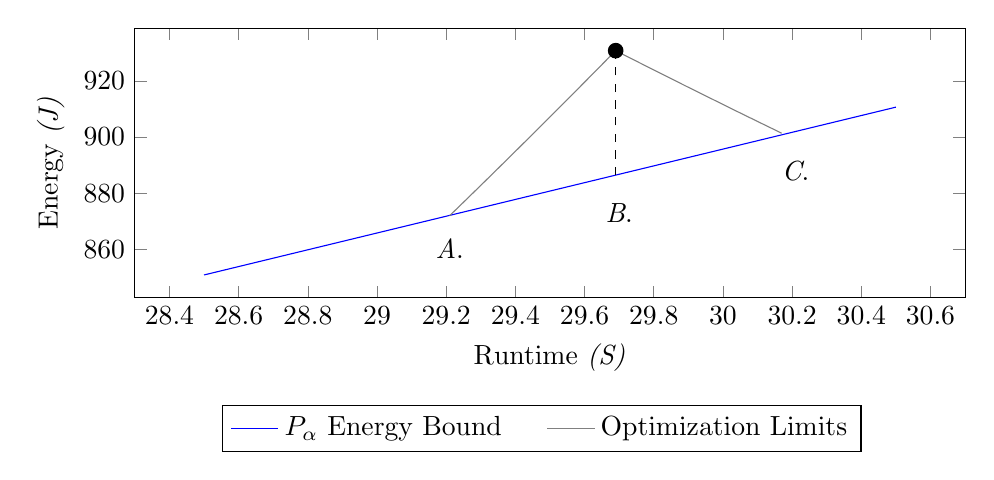
\begin{tikzpicture}
  \begin{axis}[no markers, ylabel={Energy \emph{(J)}}, xlabel={Runtime \emph{(S)}}, axis on top,
    width=\linewidth,
    height=5cm,
    legend style={at={(0.49,-0.4)}, anchor=north,legend columns=2, /tikz/every even column/.append style={column sep=0.5cm}}
    ]

    \pgfmathsetmacro{\baseline}{29.857} % NOP code

    %code, power, time
    %cfd, 31.348872, 29.689872
    %heartwall, 32.072718, 24.456485
    %lavaMD,  32.715703, 65.387028
    %leukocyte, 30.771108, 38.950881
    %streamcluster, 32.192283, 33.801999


     \addplot[domain=28.5:30.5, blue] {\baseline * x};
     \addlegendentry{$P_{\alpha}$ Energy Bound} 

  
     %% CFD %%
     \pgfmathsetmacro{\cfdpower}{31.348872}
     \pgfmathsetmacro{\cfdtime}{29.689872}
     \pgfmathsetmacro{\cfdenergy}{\cfdpower * \cfdtime}
     \pgfmathsetmacro{\baseenergy}{\baseline * \cfdtime}
     \addplot[domain=\cfdtime:30.17, gray, forget plot] { (\cfdpower * \cfdtime^3) / ((x)^2)};
     \addplot[domain=29.21:\cfdtime, gray] { (\cfdpower / \cfdtime^3) * x^4}; % Power time same ratio

     \node[circle,fill,inner sep=2pt] at (axis cs:\cfdtime, \cfdenergy) {};
     \addlegendentry{Optimization Limits} 

    \draw[dashed] ({axis cs:\cfdtime,0}|-{axis cs:0,\baseenergy}) -- ({axis cs:\cfdtime,0}|-{axis cs:0,\cfdenergy});
    
    \node at (axis cs:29.21,860) {\textit A.};                                   
    \node at (axis cs:29.7,873) {\textit B.};                                   
    \node at (axis cs:30.21,888) {\textit C.};                                   



%     %% CFD %%
%     \addplot[domain=39:48, gray] { (\sedtargetenergy * \sedtargetseconds *  \sedtargetseconds) / ((x)^2)};
%     \addplot[domain=33:41, gray] { (\sedtargetpower / \sedtargetseconds^3) * x^4}; % Power time same ratio
%     \addlegendentry{$ED^{2}P$} 
 

    
      
 \end{axis}
\end{tikzpicture}

\caption{Power Heuristic for Rodinia CFD}
\end{figure}

	
	

We first construct a power model in the vein of those proposed in the literature. We then try to link the predictions of our model to the power equations given previously. Essentially we are attempting to test against the null hypothesis - to show how much better or worse our regressed model is better than a naive attempt.


\fragment{this tent shaped region}
\fragment{Despite its simplicity, this simple model provides us with lots of information. \todo{biggest gain to be had by using power vs classical optimization, energy reduction possible through power optimization ignoring any runtime effects, the maximum amount of time we can trade for any gains in energy efficiency, and a convenient way of comparing different codes}}




\fragment{Often power models are assessed by their performance relative to a measured baseline. Although this is important, this figure is somewhat meaningless without context. Our approach is one of quantifying 


\todo{Make this bit less attacky:}
It is also worth noting that this model is effectively useless from a code optimization standpoint as it does not take any software features into account. This property is intentional, as it allows us once again to provide a baseline from which to assess any models. One can only realistically expect to optimize a code to the level at which any changes can be accurately measured. A model which claims to assist in the optimization of codes can only offer optimizations to the extent it shows divergence from this baseline.

}


\fragment{The unknown quantities in our simplified power equations can be empirically measured. \todo{Occam's razor - stronger than regression if not out performed by it}}



\fragment{Accuracy figures without context are notoriously unreliable. To compensate for this we compare the outputs of various models against a baseline we have devised. This baseline consists of what we regard as the simplest non-trivial power model conceivable. This model stands in as a sort of null hypothesis test, our justification being that a complex model only adds value to the extent with which it outperforms this toy model.}

\fragment{Our toy model is not the simplest model possible - It is well established and readily apparent that runtime is the largest contributory factor to power consumption. One could therefore imagine a simple power model}

\fragment{We consider this to be the absolute minimum power consumption possible.}

\fragment{Intentionally simplistic. Our decision to simplify activity factor to active cores is part of this. We assume that instruction pipe-lining does a reasonable job of keeping as much silicon active as possible, and we do not know how much area an individual instruction activates, and a large percentage of power use is from clock circuitry anyway}



\fragment{Two components to our investigation. Firstly, the upper bound imposed by the baseline power consumption. Secondly, as we can only view power figures approximately, the error introduced into these models necessarily limits their usefulness as optimization tools beyond a certain point.}







\todo{table 2 - micro-benchmark results. Linpack is 35.2428 for 100 seconds}
\todo{Something about how any delta is about how the code uses more logic elements than our NOP lo ops. Our optimization window is therefore within that Delta}

\todo{Be nice, say that this does not invalidate other work, but simply shows that hardware has now reached \reword{convergence} and basically there's little traction left}

Having shown that 

\fragment{This model is not supposed to be rigorous or precise. Rather we present it as the simplest possible non-trivial power model which accounts for the sources of variability in the power equations. In effect our model is functionally equivalent to the power equations
presented previously with appropriate constants substituted \todo{sampled}. We present this model as our null hypothesis - for a model to be useful it must outperform this one. It is necessarily an oversimplification - it ignores clock gating. It should also consistently underestimate the true value, as the benchmark selected intentionally exercises the minimum possible number of logic elements while still performing work.}


\todo{One limitation of this work stems from the nature of RAPL - it is an accumulative measurement of power taking into account all processes. On a loaded system it will measure all tasks }

\begin{figure}
\label{fig:dummy_model}
\includegraphics[width=0.9\linewidth]{./Plots/dummy_model/dummymodel-figure0.pdf}
\caption{Feasible Performance Envelope}
\end{figure}

\todo{Decompose the model - find baseline vs non-baseline components}
\todo{This kind of shows us that the baseline dominates}

\fragment{Limitations to optimizations - the superfluous and the logical equivalences. The first is a no-brainer and boils down to removing unnecessary pre-fetching}

\fragment{Either optimizations which are off the critical path, or else those which are on the critical path }

\fragment{Put another way, any optimization which trades runtime for power has a limited window of}

\todo{equationify fact that energy is power * time, and assume we have power decreases, time static or increases}
\todo{equationify baseline lt optimized lt unoptimized lt roofline} \todo{note - roofline is tdp max}

\todo{Do maths think - by what margin would power have to go down to justify longer runtime? ratio of cost per watt, amortized cost per second}

Nothing discussed so far precludes power optimization in practice.
\todo{imply limits thus far are theoretical}
Even these tight limits may still admit some benefits at extreme scale.
Our final argument however is strictly economic.
\reword{A great deal of attention is paid to the fact that power costs are approaching parity with machine construction costs.} The \choice{implicit, unspoken} \choice{consequence, corollary, implication} being that this has not yet happened. \todo{Ultimate point being here the price difference, machine vs power cost places a further limit on optimization utility. Even if we manage to find a slower, more power efficient method of computing a given result, the cost of energy saved has to be less than the added amortized runtime cost.}


\todo{Legitimate targets for optimization: removing redundant prefetch operations as per phi paper.}
